\documentclass[11pt,a4paper]{article}

\usepackage[margin=1in]{geometry}
\usepackage{booktabs}
\usepackage{hyperref}
\usepackage{graphicx}
\usepackage{tikz}
\usetikzlibrary{positioning,arrows.meta}
\usepackage{url}
\usepackage{enumitem}
\usepackage{xcolor}

\title{From Manual to Evidence-Based CVSS Environmental Assessment:\\
A Multi-Agent Automation Case Study with AI Bridge}

\author{
Wagner Santos \and
[Co-authors to be completed]
}

\date{\today}

\begin{document}
\maketitle

\begin{abstract}
Environmental metrics in the Common Vulnerability Scoring System (CVSS) allow
assessors to adapt vulnerability severity to the deployment context of an
organization. Prior empirical work showed that human assessment of these
metrics becomes error-prone as network segmentation and system dependencies
increase. This paper proposes an evidence-based automation workflow using AI
Bridge, a local multi-agent execution framework that can read environment
files, run controlled commands, coordinate independent agent reviews through
watchers, and produce auditable CVSS Environmental assessments. We present a
PCI-DSS inspired case study in which AI agents replace human subjects and
derive environmental metrics from structured evidence: asset inventory, network
topology, firewall rules, business impact, PCI scope and vulnerability findings.
The expected contribution is not an autonomous replacement for expert judgment,
but a reproducible and auditable process for generating CVSS Environmental
vectors with explicit evidence and review traces.
\end{abstract}

\section{Introduction}

The Common Vulnerability Scoring System (CVSS) is widely used to communicate
the severity of software vulnerabilities. In practice, however, organizations
often rely on the Base score only, even though the real operational severity of
a vulnerability depends on local deployment conditions, business criticality,
security requirements, and mitigating controls.

A previous controlled experiment on CVSS Environmental Metrics showed that
manual assessment does not scale well with environmental complexity. In that
study, assessors were more accurate in a flat network than in a segmented
network, and system-level vulnerabilities were harder to assess correctly than
application-level vulnerabilities in segmented environments~\cite{allodi2017cvssenv}.
The study concluded that automation and data integration are necessary for
environmental assessments to become practical at organizational scale.

This paper continues that line of research. Instead of running another human
subject experiment, we investigate whether a local multi-agent automation
framework can perform the environmental assessment task by collecting and
reasoning over evidence. We use AI Bridge as the execution substrate. AI Bridge
can read local files, run controlled commands, coordinate messages through a
watcher, relay tasks across chats or agents, and produce auditable artifacts.

The main research question is:

\begin{quote}
Can tool-augmented AI agents, operating through AI Bridge, generate reproducible
and evidence-backed CVSS Environmental assessments for segmented PCI-DSS-like
environments?
\end{quote}

\section{Background}

\subsection{CVSS Environmental Metrics}

CVSS version 4.0 organizes vulnerability scoring into Base, Threat,
Environmental and Supplemental metric groups~\cite{firstcvss40}. The Base
metrics describe intrinsic properties of a vulnerability, while Environmental
metrics are intended to adapt severity to the consumer's environment. The NVD
provides CVSS calculators and supports CVSS v4.0, but environmental assessment
depends on local organizational context~\cite{nvdcvss,nvdcvss40support}.

This artifact initially implements CVSS v3.1 Environmental scoring because it
is directly comparable with the previous CVSS 3.x experimental setup. The
workflow focuses on security requirements (CR, IR, AR) and selected Modified
Base metrics such as Modified Attack Vector (MAV). The paper positions CVSS
v4.0 support as the next natural extension.

\subsection{PCI-DSS Scope and Vulnerability Prioritization}

PCI-DSS scoping separates systems that process or can interact with cardholder
data from systems outside the cardholder data environment. In the original
experiment, the same conceptual model was used to test whether assessors could
correctly adapt Environmental metrics before and after segmentation.

\section{Related Work and Gap}
\label{sec:related}

CVSS is the reference scoring vocabulary for many vulnerability-management workflows. CVSS v3.1 organizes metrics into Base, Temporal, and Environmental groups, while CVSS v4.0 reorganizes the model into Base, Threat, Environmental, and Supplemental groups. This distinction is important for the present work because Base metrics describe intrinsic vulnerability properties, whereas Environmental metrics describe characteristics that are unique to the consumer's deployment environment \cite{firstcvss31,firstcvss40}. The official CVSS v4.0 specification explicitly recommends enriching Base metrics with Threat and Environmental values when the consumer needs a score that better reflects organizational risk context \cite{firstcvss40}.

Public vulnerability data sources do not usually solve this environmental-assessment problem for the consumer. The NVD provides CVSS enrichment for published CVE records, but its assessment is primarily based on Base metrics and it does not currently provide Environmental, Threat, or Supplemental metric assessments for a specific consuming organization \cite{nvdmetrics}. This creates the operational gap addressed by this paper: the information needed for environmental scoring is normally local to the organization, distributed across asset inventory, topology, firewall rules, business impact, and compliance scope.

Alternative prioritization frameworks address related but different problems. SSVC structures vulnerability response as a stakeholder-specific decision process, reducing reliance on one-size-fits-all scoring and emphasizing decisions that match the stakeholder's context \cite{ssvc2021,cisassvc}. EPSS estimates the probability that a vulnerability will be exploited in the wild, providing a threat-likelihood signal that complements severity scoring \cite{epss2021,firstepss}. These approaches are useful for prioritization, but they do not by themselves derive CVSS Environmental metrics such as security requirements or modified attack vector from local network evidence.

Prior environmental-scoring work is closest to the present study. Eitel proposed Environmental Aware Vulnerability Scoring, arguing that Environmental metrics are frequently ignored and that systematic automation requires information about systems and networks represented in a model \cite{eitel2020environmental}. The present work follows the same evidence-integration premise but uses the AI Bridge watcher as an execution and audit layer: it can read structured local artifacts, coordinate specialized review roles, regenerate outputs, and preserve an inspectable trace.

Recent work on language models and vulnerability scoring has focused mainly on automated CVSS prediction from vulnerability descriptions. AutoCVSS evaluates LLMs for automated software vulnerability scoring \cite{sanvito2025autocvss}, and EvalSVA studies multi-agent evaluators for software vulnerability assessment \cite{wen2025evalsva}. These systems are relevant because they show that LLMs and multi-agent designs can support vulnerability assessment tasks. However, their primary input is vulnerability text or code-related evidence, not organization-specific environmental artifacts. The remaining gap is therefore a reproducible workflow that connects local environmental evidence to CVSS Environmental metrics and records why each metric value was selected.

\section{AI Bridge Approach}

AI Bridge is used as a local execution and orchestration layer. The intended
workflow is shown in Figure~\ref{fig:pipeline}.

\begin{figure}[ht]
\centering
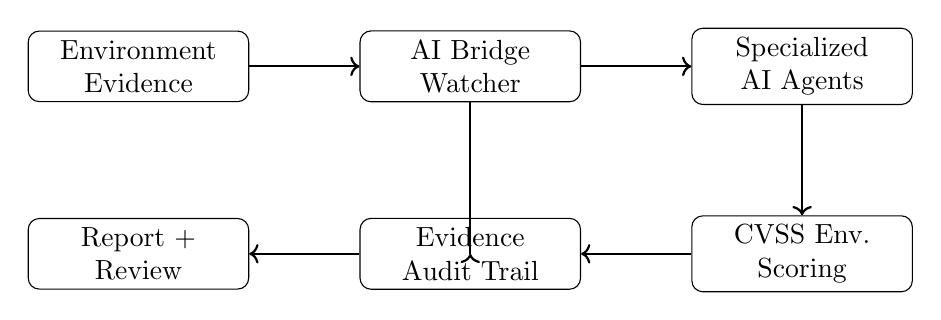
\begin{tikzpicture}[
  node distance=1.4cm,
  block/.style={draw, rounded corners, align=center, minimum width=2.8cm, minimum height=0.8cm},
  arrow/.style={->, thick}
]
\node[block] (inputs) {Environment\\Evidence};
\node[block, right=of inputs] (watcher) {AI Bridge\\Watcher};
\node[block, right=of watcher] (agents) {Specialized\\AI Agents};
\node[block, below=of agents] (scoring) {CVSS Env.\\Scoring};
\node[block, left=of scoring] (audit) {Evidence\\Audit Trail};
\node[block, left=of audit] (report) {Report +\\Review};

\draw[arrow] (inputs) -- (watcher);
\draw[arrow] (watcher) -- (agents);
\draw[arrow] (agents) -- (scoring);
\draw[arrow] (scoring) -- (audit);
\draw[arrow] (audit) -- (report);
\draw[arrow] (watcher) |- (audit);
\end{tikzpicture}
\caption{Evidence-based CVSS Environmental assessment workflow using AI Bridge.}
\label{fig:pipeline}
\end{figure}

We define four agent roles:
\begin{enumerate}[noitemsep]
  \item Network/Topology Analyst;
  \item PCI-DSS Scope Reviewer;
  \item CVSS Environmental Analyst;
  \item Evidence Consolidator.
\end{enumerate}

The agents do not simply output a score. Each metric value must reference
evidence, such as asset inventory, business impact classification, firewall
rules, topology, or vulnerability metadata.

\section{Case Study Design}
\label{sec:case-study}

The case-study design follows the logic of the prior PCI-DSS inspired experiment:
compare environmental assessment under flat and segmented network conditions. The
new study adds machine-readable evidence artifacts so that the same type of
scenario can be assessed by deterministic scripts, language-model agents, and a
watcher-enabled multi-agent workflow.

Each case is represented by:
\begin{itemize}[leftmargin=*]
  \item an asset inventory;
  \item vulnerability findings;
  \item network topology;
  \item firewall rules;
  \item business-impact mappings;
  \item PCI scope declarations; and
  \item expected expert labels used only for evaluation.
\end{itemize}

The experimental comparison includes four conditions:
\begin{enumerate}[leftmargin=*]
  \item historical human-baseline findings from the prior study;
  \item a deterministic rule-based baseline;
  \item a language-model baseline without local tool access; and
  \item the AI Bridge watcher workflow with local evidence access.
\end{enumerate}

The main outcomes are exact match against expert labels, environmental score
error, correct direction of before-after change, reproducibility across repeated
runs, and evidence coverage. Evidence coverage is defined as the proportion of
scoring decisions that can be traced to a concrete artifact such as an asset
record, topology entry, firewall rule, PCI scope declaration, or business-impact
statement.

\section{Artifact and Implementation}

The artifact is organized as a reproducible starter kit. The Python application
loads structured case files, applies transparent inference rules, computes CVSS
v3.1 Environmental scores, and writes JSON, CSV, JSONL and Markdown outputs.

The AI Bridge folder contains watcher command templates and agent prompts. These
files are intended to operationalize the case study through real AI Bridge
execution: local file reading, command execution, chat-to-chat review, and
evidence consolidation.

The artifact produces an \texttt{audit\_trace.jsonl} file where each line links a
metric decision to a source and a reason. This is the core mechanism that turns
the assessment from an opaque AI output into an auditable procedure.

\section{Artifact Validation and Baseline Results}
\label{sec:evaluation}

The current artifact includes a clean deterministic validation run for the PCI segmented lab case. The run is stored in \path{outputs/runs/pci_segmented_lab_20260517_143146/} and is accompanied by \path{run_manifest.json}, input hashes, generated assessments, an audit trace, and a before-after comparison table. These results are treated as artifact-validation results, not as evidence that the watcher workflow outperforms human experts. The evaluation scope is deliberately conservative: it checks reproducibility, traceability, data completeness, label consistency, and dashboard readiness for the deterministic baseline before any broader human-subject or watcher-mediated comparison is claimed. The evaluation scope is deliberately conservative: it checks reproducibility, traceability, data completeness, label consistency, and dashboard readiness for the deterministic baseline before any broader human-subject or watcher-mediated comparison is claimed.


The before-after comparison is summarized in Table~
\
ref{tab:env-effects}. The table is generated from the deterministic run artifacts rather than from manual transcription, so it also acts as a compact reproducibility check for the dashboard and manuscript pipeline.


\
begin{table}[htbp]

\
centering

\
caption{Environmental-score effects in the deterministic PCI segmented lab baseline.}

\
label{tab:env-effects}

\
begin{tabular}{llllrrr}

\
hline
Finding & Asset & CVE & Effect & Before & After & Delta 
\
\
 
\
hline
F-001 & A-CORP-SRV & CVE-2016-0036 & downgraded & 8.8 & 8.0 & -0.8 
\
\
F-002 & POS-01 & CVE-2016-0469 & unchanged & 7.8 & 7.8 & 0.0 
\
\
F-003 & ADMIN-01 & CVE-2016-3234 & downgraded & 8.8 & 8.0 & -0.8 
\
\
F-004 & WIRELESS-LEGACY-01 & CVE-2016-1619 & unchanged & 7.8 & 7.8 & 0.0 
\
\
F-005 & CORE-SW-01 & CVE-2016-6441 & unchanged & 9.7 & 9.7 & 0.0 
\
\
F-006 & CORE-SW-01 & CVE-2016-6428 & unchanged & 8.8 & 8.8 & 0.0 
\
\
 
\
hline

\
end{tabular}

\
end{table}
The run generated 12 assessments for six findings, with one before and one after segmentation assessment per finding. All generated CR, IR, AR, and MAV labels matched the expected expert labels included in the structured case files. Two findings were downgraded after segmentation, four remained unchanged, and none were upgraded. The mean environmental-score delta was -0.267 and the maximum absolute delta was 0.8.

\begin{table}[ht]
\centering
\caption{Clean deterministic before-after run for the PCI segmented lab case.}
\label{tab:clean-run-effects}
\begin{tabular}{lllrrrrl}
\toprule
Finding & Asset & Type & MAV & Before & After & Delta & Effect \\
\midrule
F-001 & A-CORP-SRV & SYS & N--A & 8.8 & 8.0 & -0.8 & downgraded \\
F-002 & POS-01 & SYS & L--L & 7.8 & 7.8 & 0.0 & unchanged \\
F-003 & ADMIN-01 & APP & N--A & 8.8 & 8.0 & -0.8 & downgraded \\
F-004 & WIRELESS-LEGACY-01 & APP & N--N & 7.8 & 7.8 & 0.0 & unchanged \\
F-005 & CORE-SW-01 & SYS & A--A & 9.7 & 9.7 & 0.0 & unchanged \\
F-006 & CORE-SW-01 & SYS & A--A & 8.8 & 8.8 & 0.0 & unchanged \\
\bottomrule
\end{tabular}
\end{table}

The final evaluation will compare four conditions: historical human baseline, deterministic rule-based baseline, language-model baseline without local tool access, and AI Bridge watcher-mediated multi-agent assessment with local evidence access. The primary metrics are exact match for CR, IR, AR, and MAV; secondary metrics include environmental-score error, correct before-after direction, reproducibility across repeated runs, evidence coverage, and audit-trace completeness.





The broader engineering-validation set is summarized in Table~
\
ref{tab:curated-runs}. These additional scenarios are curated case packages used to exercise the deterministic pipeline and artifact summarizer. They extend engineering coverage, but they are not yet treated as independent comparative evidence because external expert review and arm-level adjudication remain future study steps.


\
begin{table}[htbp]

\
centering

\
caption{Curated run summary for deterministic engineering validation.}

\
label{tab:curated-runs}

\
begin{tabular}{lrrrrr}

\
hline
Run & Findings & Assessments & Down & Same & Up 
\
\
 
\
hline
pci_segmented_lab & 6 & 12 & 2 & 4 & 0 
\
\
pci_demo_curated & 10 & 20 & 0 & 10 & 0 
\
\
complex_curated & 10 & 20 & 0 & 10 & 0 
\
\
 
\
hline

\
end{tabular}

\
end{table}

Automated watcher IA validation scope. The current validation workflow is automated and watcher mediated. The pipeline generates evidence linked review rows and reports under validation/ai_review from committed curated artifacts. It does not claim completed independent human expert adjudication. Human expert review is treated as future comparative work rather than a dependency for the present evaluation.


Automated watcher IA validation summary table. 
Automated watcher IA validation outputs were not found during this run.


The automated validation summary table is generated from committed artifacts in article/generated/automated_validation_summary_table.txt and docs/generated/automated_validation_article_inputs.md. It reports watcher IA validation counts and explicitly excludes independent human adjudication claims.


Multi-scenario deterministic pipeline results. The current artifact package includes 
1
 curated scenarios, 
6
 findings, and 
12
 automated environmental CVSS assessments. The deterministic engine classified 
2
 assessments as downgraded, 
4
 as unchanged, and 
0
 as upgraded. These values are generated from committed scenario artifacts and automated watcher IA validation outputs, not from completed independent human expert adjudication.


Trace-enabled evaluation artifacts. The generated comparison CSV files now include per-assessment adjustment traces. This supports inspection of why a finding was downgraded, unchanged, or upgraded under the current prototype scoring policy.


Results package artifacts. The current results package includes curated run summaries, automated watcher IA validation summaries, and adjustment trace summaries. These artifacts provide the basis for the reported scenario totals, decision counts, and traceability claims.


\section{Threats to Validity}

The main construct validity risk is that structured case files may simplify real
enterprise environments. This is mitigated by explicitly representing topology,
scope, firewall rules, business impact and vulnerability metadata.

The main internal validity risk is that rule-based inference may encode the
expert judgment instead of discovering it. For this reason, the multi-agent
version should be executed separately and compared to the expert label file.

The main external validity risk is that one PCI-DSS-inspired case may not
represent other regulated environments. The artifact is therefore designed to
allow additional case folders.

\section{Conclusion}

This paper proposes a continuation of prior empirical work on the difficulty of
CVSS Environmental assessment. The central claim is that the next step is not
another purely manual study, but an evidence-based automation workflow that
allows AI agents to collect, interpret, justify and audit environmental metric
decisions.

AI Bridge provides the operational substrate for this workflow: local file access,
controlled command execution, watcher-mediated agent coordination, and artifact
generation. The initial case study and Overleaf template included in this package
provide the starting point for a full paper and reproducible research artifact.


\bibliographystyle{plain}
\bibliography{references}

\appendix
\section{Artifact Manifest}

\begin{itemize}[noitemsep]
  \item \texttt{app/}: Python prototype for deterministic environmental assessment.
  \item \texttt{cases/pci\_segmented\_lab/}: structured PCI-DSS-inspired case.
  \item \texttt{ai\_bridge/}: watcher envelopes, prompts and evidence schema.
  \item \texttt{outputs/demo\_run/}: example generated outputs.
  \item \texttt{tex/}: Overleaf-ready article template.
\end{itemize}

The artifact can be executed with:

\begin{verbatim}
python app/run_demo.py --case cases/pci_segmented_lab --out outputs/demo_run
\end{verbatim}


\end{document}
